% !TEX TS-program = pdflatex
% !TEX encoding = UTF-8 Unicode

% This is a simple template for a LaTeX document using the "article" class.
% See "book", "report", "letter" for other types of document.

\documentclass[11pt]{article} % use larger type; default would be 10pt

\usepackage[utf8]{inputenc} % set input encoding (not needed with XeLaTeX)


%%% PAGE DIMENSIONS
\usepackage{geometry} % to change the page dimensions
\geometry{a4paper} % or letterpaper (US) or a5paper or....


\usepackage{graphicx} % support the \includegraphics command and options

% \usepackage[parfill]{parskip} % Activate to begin paragraphs with an empty line rather than an indent

%%% PACKAGES
\usepackage{booktabs} % for much better looking tables
\usepackage{array} % for better arrays (eg matrices) in maths
\usepackage{paralist} % very flexible & customisable lists (eg. enumerate/itemize, etc.)
\usepackage{verbatim} % adds environment for commenting out blocks of text & for better verbatim
\usepackage{subfig} % make it possible to include more than one captioned figure/table in a single float
\usepackage{cite}
% These packages are all incorporated in the memoir class to one degree or another...

%%% HEADERS & FOOTERS
\usepackage{fancyhdr} % This should be set AFTER setting up the page geometry
\pagestyle{fancy} % options: empty , plain , fancy
\renewcommand{\headrulewidth}{0pt} % customise the layout...
\lhead{}\chead{}\rhead{}
\lfoot{}\cfoot{\thepage}\rfoot{}

%%% SECTION TITLE APPEARANCE
\usepackage{sectsty}
\allsectionsfont{\sffamily\mdseries\upshape} % (See the fntguide.pdf for font help)
% (This matches ConTeXt defaults)

%%% ToC (table of contents) APPEARANCE
\usepackage[nottoc,notlof,notlot]{tocbibind} % Put the bibliography in the ToC
\usepackage[titles,subfigure]{tocloft} % Alter the style of the Table of Contents
\renewcommand{\cftsecfont}{\rmfamily\mdseries\upshape}
\renewcommand{\cftsecpagefont}{\rmfamily\mdseries\upshape} % No bold!

\title{Mapping the Brain: An Introduction to Connectomics\\Extracting Novel Biological Priors from Neuronal Skeletons for Classification}
\author{Katie Link, Elizabeth Morgan, Sandra Weiss}
%\date{} % Activate to display a given date or no date (if empty),
         % otherwise the current date is printed 

\begin{document}
\maketitle

\section{Abstract}
	With recent advances in big data storage and image processing, the extraction of connectomes from electron microscopy (EM) images, whose volume of neurons are often converted to and visualized as neuronal skeletons, has become much more feasible. Producing a connectome provides an informative graph of the connections between neurons in the brain. However, despite the large amounts of data available, a  system of automatically classifying the different neuron trees by looking at their differences in biological priors has not been fully developed or explored. This project attempts to compare two specific types of hippocampal neurons, pyramidal cells and granule cells, found in rats. The priors that were looked at included branch length, branch order, path length, branch angle, number of tips, and number branches. Using neuron skeletons provided by NeuroMorpho.org and the TREES toolbox for MATLAB, the means and standard deviations were calculated for granule cells and pyramidal cells, histogram plots using the kernal smoothing function estimate and comparing the priors of the two neurons were created, and the statistical difference was calculated using the Hellinger distance. Although this project ended here, in the future, the differences between the priors of these two neurons could be meaningful when being used to improve the accuracy and speed of neuron classification during connectome extraction.

\section{Results}
	All six priors show promise a classification tools for neuronal skeletons. After computing the statistical difference using the Hellinger distance, five of the six priors had p-values of 0. Branching angle, which had a p-value of 0.0161, also had very close means (81.9521 degrees in the granule cells and 80.0280 degrees in the pyramidal cells, and therefore would probably be the worst classifier between granule and pyramidal cells (see figure 1).\\
\\
	Branching order, number of tips, and number of branches, on the other hand, showed great difference both visually in their plots (see figures 2, 3, and 4) as well as in their means and standard deviations. These three priors, therefore, would be an appropriate starting point for a machine-learning-based classification pipeline.\\
\\
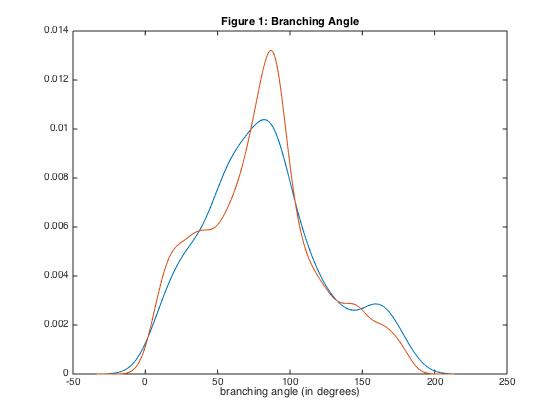
\includegraphics[width=0.5\textwidth]{Figure_1.jpg}
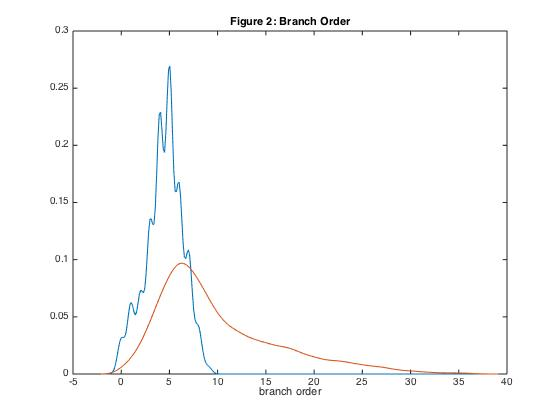
\includegraphics[width=0.5\textwidth]{Figure_2.jpg}
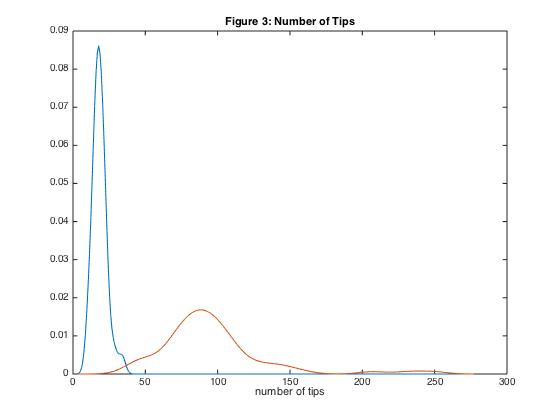
\includegraphics[width=0.5\textwidth]{Figure_3.jpg}
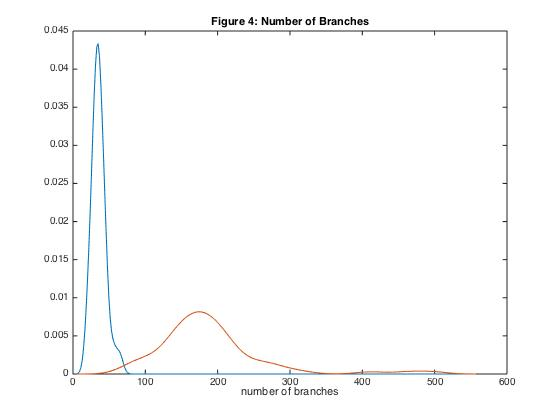
\includegraphics[width=0.5\textwidth]{Figure_4.jpg}


\end{document}